\documentclass{article}	
\usepackage{tikz}
\tikzset{near start abs/.style={xshift=1cm}}
\usetikzlibrary{calc}
\usetikzlibrary{intersections}
\usetikzlibrary{arrows.meta,quotes}
\usepackage{siunitx}

\begin{document}


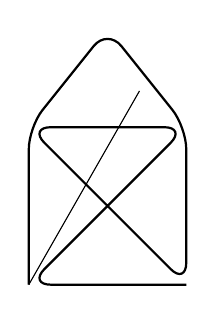
\begin{tikzpicture}
	\draw (0pt,0pt) -- (40pt,70pt);
	\draw[thick,rounded corners=8pt]
(0,0) -- (0,2) -- (1,3.25) -- (2,2) -- (2,0) -- (0,2) -- (2,2) -- (0,0) -- (2,0);


\end{tikzpicture}

\vspace{1cm}

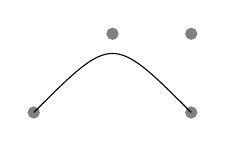
\begin{tikzpicture}
\filldraw [gray] (0,0) circle [radius=2pt]
(1,1) circle [radius=2pt] (2,1) circle [radius=2pt] (2,0) circle [radius=2pt];
  \draw (0,0) .. controls (1,1) .. (2,0);
\end{tikzpicture}

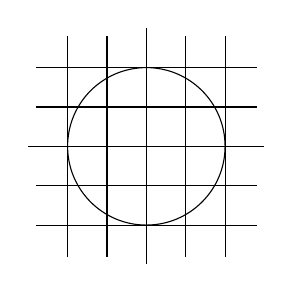
\begin{tikzpicture}


\draw[step=.5cm] (-1.4,-1.4) grid (1.4,1.4); \draw (-1.5,0) -- (1.5,0);
\draw (0,-1.5) -- (0,1.5);
\draw (0,0) circle [radius=1cm];
\tikzset{help lines,color=blue!50,very thin}

\end{tikzpicture}

\tikzset{Karl's grid/.style={help lines,color=blue!50}}

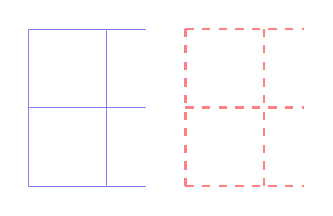
\begin{tikzpicture}
[Karl's grid/.style ={help lines,color=#1!50}, Karl's grid/.default=blue]

\draw[Karl's grid]     (0,0) grid (1.5,2);
\draw[Karl's grid=red, thick, dashed] (2,0) grid (3.5,2); 
\end{tikzpicture}

\begin{figure}[h]
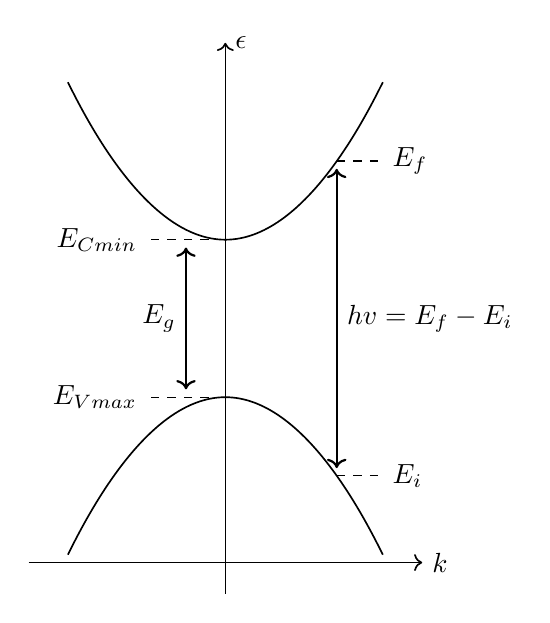
\begin{tikzpicture}
	\draw[semithick] (-2,3) parabolabend (0,1) (2,3);
	\draw[semithick] (-2,-3) parabolabend (0,-1) (2,-3);
	\draw[<-,semithick] (0,3.5) -- (0,-3.5) node[anchor=west, pos=0] {$\epsilon$} ; % y axis
	\draw[->, semithick] (-2.5,-3.1) -- (2.5,-3.1) node[anchor=west, pos=1] {$k$} ; % x axis
	\draw[dashed] (0,1) -- (-1,1) node[anchor=east] {$E_{Cmin}$};
	\draw[dashed] (0,-1) -- (-1,-1) node[anchor=east] {$E_{Vmax}$};
	\draw[<->, thick] (-0.5,-0.9) -- (-0.5,0.9) node[anchor=east, midway] {$E_{g}$};
	\draw[dashed] (1.414,2) -- (2,2) node[anchor=west] {$E_{f}$};
	\draw[dashed] (1.414,-2) -- (2,-2) node[anchor=west] {$E_{i}$};
	\draw[<->, thick] (1.414,-1.9) -- (1.414,1.9) node[anchor=west, midway] {$hv = E_f-E_i$} ;
\end{tikzpicture}
\end{figure}

\begin{tikzpicture}[scale=2]
\clip (-2,-2) rectangle (2,2);
\draw[step=.5cm,help lines] (-1.4,-1.4) grid (1.4,1.4); \filldraw[fill=green!20,draw=green!50!black] (0,0) -- (3mm,0mm)
arc [start angle=0, end angle=30, radius=3mm] -- cycle; \draw[->] (-1.5,0) -- (1.5,0); \draw[->] (0,-1.5) -- (0,1.5); \draw (0,0) circle [radius=1cm];
\foreach \x in {-1,-0.5,1}
\draw (\x cm,1pt) -- (\x cm,-1pt) node[anchor=north] {$\x$};
\foreach \y in {-1,-0.5,0.5,1}
\draw (1pt,\y cm) -- (-1pt,\y cm) node[anchor=east] {$\y$};
\end{tikzpicture}

\begin{tikzpicture}
    % place nodes
    \node[draw] at (0, 0)   (a) {A};
    \node[draw] at (3, 0)   (b) {B};

    \node[draw] at (0, -2)  (c)     {C};
    \node[draw] at (5, -2)  (d)     {D};

    % draw edges
    \draw[] (a) node[above,xshift=2cm] {$x(kT)$} -- (b);
    \draw[] (c) node[above,xshift=1cm] {$y(kT)$} -- (d);
    \draw (0,-3) node[above,near start abs] {Test} -- ++(7,0);
\end{tikzpicture}

\vspace{3cm}
\begin{tikzpicture}[auto,bend right]
  \node (a) at (-2,3) {};
  \node (b) at (0,1) {};
  \node (c) at (2,3) {};
  \node (p1) at (-3,-3) {};
  \node (p2) at (0,-1) {};
  \node (p3) at (3,-3) {};
  \draw[->] (a) parabola bend (b) (c) coordinate[pos=0.5](A);
  \draw[->] (p1) parabola bend (p2) (p3) coordinate[pos=0.5](B);
  \coordinate (b1) at ($ (b)!.5!(c) $);
  \coordinate (b2) at ($ (p2)!.33!(p3) $);
  \draw [<->] (b1) -- (b2) node [sloped,midway,above] {1cm};
  \draw [<->] (A) -- (B) node {1cm};
\end{tikzpicture}

 \begin{tikzpicture}
    \coordinate (1) at (-3,-3);
    \coordinate (2) at (3,3);
    \coordinate (O) at (0,0);

    \draw (-1.5,-3) node[below]{directrix};
    \draw (-1.5,-3.4) node[below]{$x=-a$};
    \path (O) node[below left]{$(0,0)$} node[above left]{$V$};
    \draw [fill=black] (1,0) coordinate (F) circle (1.5pt)
     node[below]{$F(a,0)$};
    \draw[thick, ->] (-3,0) -- (5,0) node[right]{$x$};
    \draw[thick, ->] (0,-3) -- (0,3) node[above]{$y$};
    \draw[dashed,very thin] (-1.3,-3)--(-1.3,3);
    \draw (-2,4) parabola bend (0,0) (2,4);
    \path (-1.3,1.3) -- (current bounding box.east|-0,1.3);
    %\draw (-1.3,1.3) node[above left]{$N$} -- (i1) node[below right]{$P(x,y)$} -- (F);
\end{tikzpicture}

\begin{figure}[h]
\begin{tikzpicture}
	\draw[semithick] (-2,3) parabolabend (0,1) (2,3);
	\draw[semithick] (-3,-3) parabolabend (0,-1) (3,-3);

	\draw[<->, thick, shorten >=5pt, shorten <=5pt] (1.414,-1.4) -- (1.414,1.9) node[anchor=west, midway] {} ;
\end{tikzpicture}
\end{figure}
 
\begin{tikzpicture}[auto, > = Straight Barb, samples = 51]
\draw[-, semithick]   plot [domain=-2:2] (\x, {+1+0.5*(\x)^2});
\draw[-, semithick]   plot [domain=-3:3] (\x, {-1-0.25*(\x)^2}); %
\draw [fill=white] (1,{-1-0.25*(1)^2}) circle (1pt);
\draw [fill=black] (1,{+1+0.5*(1)^2}) circle (1pt);
\draw (1,{-1-0.25*(0.85)^2}) coordinate (p1) node[]{};
\draw (1,{+1+0.5*(0.9)^2}) coordinate (p2) node[]{};
%\draw[<->]  (1,{-1-0.25*(0.9)^2}) to ["{1}"]((1,{1+0.5*(0.9)^2});
\draw[<->]  (p1) -- (p2) node[anchor=west, midway]{jdjd};

\end{tikzpicture}
   
\end{document}	
